\documentclass[10.5pt]{article}   %11 puntos

%Adapted from Adapted from UWA Engineering Final Year Project.


\usepackage[utf8]{inputenc}
\usepackage[x11names,dvipsnames,svgnames,table]{xcolor}

% general incantations
\usepackage[export]{adjustbox}
\usepackage{afterpage}

\usepackage{graphicx}
\usepackage{placeins}
\usepackage{pdfpages}
\usepackage{algorithm2e}
\usepackage{array}
\usepackage{booktabs}
\usepackage[most]{tcolorbox}
\usepackage{calligra}
\usepackage{caption}
\usepackage{datetime}
\usepackage{dirtytalk}
\usepackage{dsfont}
\usepackage{etex}
\usepackage{fancyhdr}
\usepackage{fix-cm}
\usepackage[T1]{fontenc}
\usepackage{textcomp,gensymb} %for \degree C symbol
\usepackage{graphicx}
\usepackage{lipsum}
\usepackage{listings}
\usepackage{transparent}
\usepackage[everyline=true,framemethod=tikz]{mdframed}
\usepackage{mparhack}
\usepackage{multicol}
\usepackage{multirow}
\usepackage{parskip}
\usepackage{lscape}
\usepackage{pdflscape}
\usepackage{pdfpages}
\usepackage{placeins}
\usepackage[document]{ragged2e}
\usepackage{rotating}
\usepackage{setspace}
\usepackage{subcaption}
\usepackage{threeparttable}
\usepackage[normalem]{ulem}
\usepackage{verbatim}
\usepackage{soul} %highlighting, strike through etc.

%Automated appendices
\usepackage[titletoc,title,header]{appendix} %advanced functionality

%language settings
\usepackage[utf8]{inputenc}
\usepackage{csquotes}

%page setup
%this where we adjust the binding offset, if relevant
\usepackage{geometry}
\geometry{left=2cm,right=2cm,top=2cm,bottom=2cm}
\usepackage{lastpage} % for page 1 of n footers

%cross referencing
\usepackage[hidelinks]{hyperref}
\usepackage{cleveref}

%maths stuff
\usepackage{amsmath}
\usepackage{mathtools}

\setcounter{secnumdepth}{5}

%lists
\usepackage{enumitem}

%working collaboratively
\usepackage[backgroundcolor=yellow]{todonotes}

% bibliography file using harvard
\usepackage[style=apa,citestyle=bwl-FU,backend=biber, sorting=nyt]{biblatex}
\bibliography{bibliography.bib} % with extension

%glossary for acronyms
\usepackage[acronym,nonumberlist,toc,section=subsection,numberedsection=nolabel]{glossaries} 
\makeglossaries

%line spacing
\linespread{1.6}


\usepackage{times}                      %Times New Roman
\usepackage{setspace}                   %Para espaciar
%\linespread{1.25}                      %Interlineado 1.5
%\singlespacing                          %Espaciado simple

\newcommand*\Heq{\ensuremath{\overset{\kern2pt LH }{=}}}
\newcommand{\Lagr}{\mathcal{L}}         %L (lagrangiano o fun de verosimilitud)
\newcommand{\indep}{\rotatebox[origin=c]{90}{$\models$}}
\newcommand{\R}{\mathbb{R}}             %Real numbers
\usepackage[utf8x]{inputenc}
%\usepackage{apacite}                    %Citas tipo apa
%\renewcommand{\thesubsection}{\thesection.\alph{subsection}}
%\usepackage{cite}
%\usepackage[left=2.5cm,right=2.5cm,top=2.5cm,bottom=2.5cm]{geometry} %Deberían ser 3 y 3 los left y right pero lo hago así para que entre mejor
%\usepackage[round]{natbib}              %Bibliografía
%\usepackage[utf8]{inputenc}
%\usepackage{amsmath}
\usepackage{mathtools}                  %Loads amsmath
\usepackage{amssymb}

\numberwithin{equation}{section}
\usepackage{hyperref}
\usepackage{color}   %May be necessary if you want to color links
 \hypersetup{
     colorlinks=false, %set true if you want colored links
     linktoc=all,     %set to all if you want both sections and sections linked
     linkcolor=blue,  %choose some color if you want links to stand out
 }
 \usepackage[spanish,es-tabla]{babel}
 \usepackage{graphicx}
 \usepackage{physics}
 %\usepackage[hidelinks]{hyperref}

\usepackage{amssymb}    %Para tener los check mark y cruces
\usepackage{pifont}     %Para tener los check mark y cruces
\newcommand{\cmark}{\ding{51}} %Para tener los check mark y cruces
\newcommand{\xmark}{\ding{55}}  %Para tener los check mark y cruces
\usepackage{float}

%Esto lo podés volar
% \usepackage{xcolor}                 %Night mode
% \pagecolor[rgb]{0,0,0} %black       %Night mode
% \color[rgb]{0.8,0.8,0.8} %grey      %Night mode

\title{QGIS}
\author{Matías Harari y Mariana Santi}
\date{2° trimestre 2021}
\setlength{\marginparwidth}{2cm}
\usepackage{setspace}
\spacing{1.2}
\usepackage{listings}
\usepackage{color}

\definecolor{dkgreen}{rgb}{0,0.6,0}
\definecolor{gray}{rgb}{0.5,0.5,0.5}
\definecolor{mauve}{rgb}{0.58,0,0.82}

\lstset{frame=tb,
  language=Java,
  aboveskip=3mm,
  belowskip=3mm,
  showstringspaces=false,
  columns=flexible,
  basicstyle={\small\ttfamily},
  numbers=none,
  numberstyle=\tiny\color{gray},
  keywordstyle=\color{blue},
  commentstyle=\color{dkgreen},
  stringstyle=\color{mauve},
  breaklines=true,
  breakatwhitespace=true,
  tabsize=3
}
\begin{document}
\renewcommand{\thesubsection}{\thesection.\alph{subsection}}

\thispagestyle{empty}
\setlength\headheight{0pt} 
\begin{center}

\begin{center}

\includegraphics[width=0.65\linewidth]{imgs/logoudesa.png}            
\end{center}	

        \vspace{0.2cm}
        {\scshape\LARGE Departamento de Economía \par}
        \vspace{0.2cm}
        {\scshape\Large Maestría en Economía\par}
        \vspace{0.4cm}

        {\Large\bfseries Herramientas computacionales - QGIS\par}
        
        \vspace{1cm}
        {\Large\itshape Matias Harari y Mariana Santi \par}


\vspace{1cm} 
\large
{2021}

\end{center}

\clearpage
\justify


%List of figures and tables, automatic from thesis.

%\tableofcontents
%\pagebreak

%Empieza el trabajo
\section*{Airbnb en Chicago}
En esta sección, se busca tener una primera aproximación para entender los determinantes del rating de los hospedajes de Airbnb en Chicago. Se utilizarán datos de la puntuación promedio por comunidad obtenida por los dueños de los alojamientos y se presentarán algunas variables que podrían explicar la puntuación promedio.

En primer lugar, en la Figura 1 se observa que la zona noreste de la ciudad de Chicago tiene una mejor puntuación promedio en sus alojamientos de Airbnb. A su vez, se ve una fuerte disparidad en el precio cobrado en promedio en las distintas comunidades de la ciudad. En principio el precio no necesariamente debería estar relacionado positivamente a la puntuación, ya que los huéspedes suelen evaluar la calidad de sus estadía en función a sus expectativas previas al viaje. \\\

\begin{figure}[H]
\centering
\begin{subfigure}{.5\textwidth}
    \centering
     \textbf{}\par\medskip
    \includegraphics[scale=0.45]{Rating.png}
    \label{fig2}
\end{subfigure}%
\begin{subfigure}{0.65\textwidth}
    \centering
     \textbf{}\par\medskip
    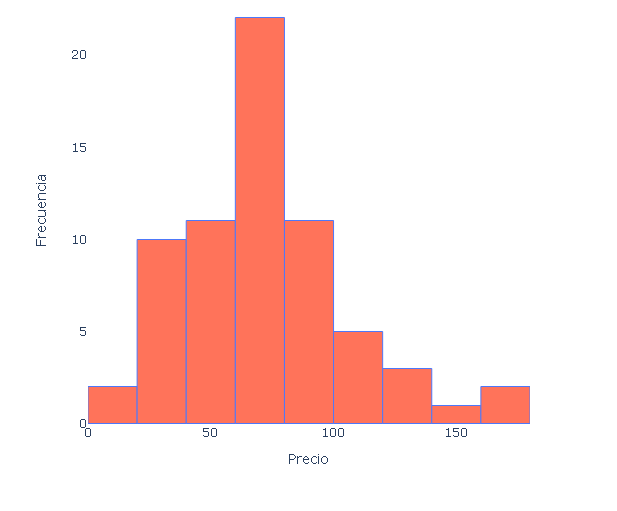
\includegraphics[scale=0.6]{Price.png}
    \label{fig2}
\end{subfigure}%
\caption{Mapa del rating de Airbnb promedio (izq.) e histograma del precio promedio de Airbnb (der.) en las comunidades de Chicago.}
\end{figure}

Por otro lado, se espera una relación positiva entre la calidad turística de la zona y la puntuación. En general, puede ser difícil para los huéspedes verificar que la zona donde se hospedan se ajusta a sus expectativas. Por ejemplo, quienes visitan por primera vez una comunidad, pueden contratar un alojamiento online porque les pareció atractivo cuando vieron las fotos, pero no suelen tomarse el tiempo o no están en condiciones de comprobar si la zona en la que se alojarán es la adecuada. Para indagar sobre esta cuestión, se presenta la Figura 2 que muestra el Harship Index de la ciudad de Chicago. Valores más altos se asocian a regiones de menores ingresos y mayor pobreza, entre otras características que indican peores indicadores socioeconómicos. Teniendo esto en cuenta, puede confirmarse que las comunidades de menor Harship Index (es decir, mejor nivel socioeconómico) suelen tener una mejor puntuación en Airbnb. Esto puede interpretarse de forma tal que los huéspedes se ven "sorprendidos" por las características de la zona y puntúan con valores más altos (bajos) a los alojamientos ubicados en regiones de mayor (menor) nivel socioeconómico. 


\begin{figure}[H]
\centering
\begin{subfigure}{.5\textwidth}
    \centering
     \textbf{}\par\medskip
    \includegraphics[scale=0.45]{Harship.png}
    \label{fig2}
\end{subfigure}%
\begin{subfigure}{0.65\textwidth}
    \centering
     \textbf{}\par\medskip
    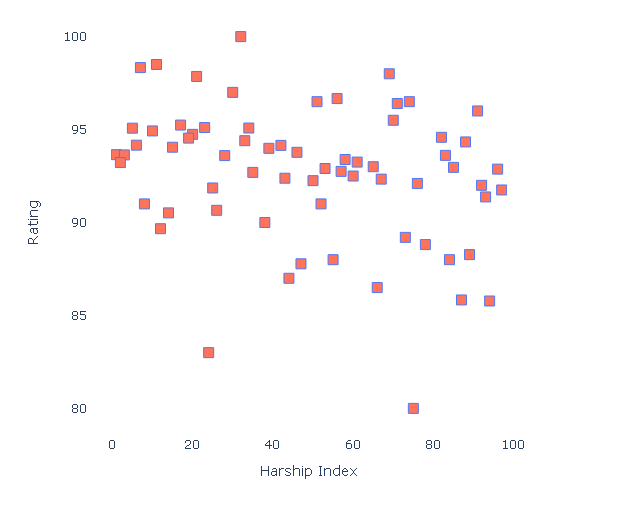
\includegraphics[scale=0.6]{Harship_Index.png}
    \label{fig2}
\end{subfigure}%
\caption{Mapa del Harship Index (izq.) y relación entre el Harship Index y el rating promedio de Airbnb (der.) en las comunidades de Chicago.}
\end{figure}

La Figura 3 muestra que la tasa de respuesta de los propietarios de Airbnb de las comunidades de Chicago no tiene demasiada variabilidad (el 50\% de las observaciones están entre 90 y 100) aunque sí existe cierta heterogeneidad espacial. A primera vista parecería que las zonas mejor puntuadas responden menos en la plataforma, aunque sería necesario controlar por otras variables para ver si efectivamente existe un efecto.

\begin{figure}[!ht]
\centering
\begin{subfigure}{.5\textwidth}
    \centering
     \textbf{}\par\medskip
    \includegraphics[scale=0.45]{Response.png}
    \label{fig2}
\end{subfigure}%
\begin{subfigure}{0.55\textwidth}
    \centering
     \textbf{}\par\medskip
    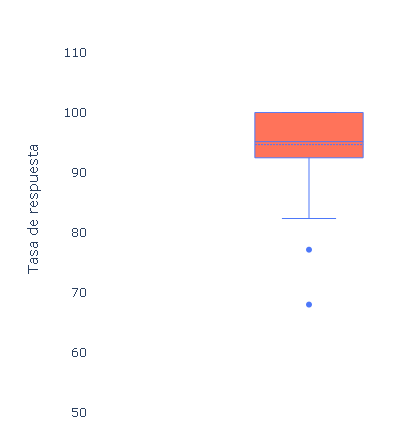
\includegraphics[scale=0.7]{Boxplot.png}
    \label{fig2}
\end{subfigure}%
\caption{Mapa de la tasa de respuesta (izq.) y boxplot (der.) de los propietarios de Airbnb de las comunidades de Chicago.}
\end{figure}

Por último, la Tabla 1 resume un breve ejercicio de inferencia causal. Allí puede confirmarse que el precio no es una variable estadísticamente significativa a la hora de explicar la puntuación de Airbnb. En cambio, sí se observa significatividad en el Harship Index, en la tasa de respuesta y en la concurrencia del alojamiento. En particular, 10 puntos más en el Harship Index reduce el rating promedio de Airbn en 0,7 puntos. Este efecto es económicamente significativo teniendo en cuenta que todos las comunidades tienen una puntuación de alojamiento promedio que se encuentra entre 8 y 10 puntos.


\begin{table}[!htbp] \centering 
  \caption{} 
  \label{} 
\begin{tabular}{@{\extracolsep{5pt}}lc} 
\\[-1.8ex]\hline 
\hline \\[-1.8ex] 
 & \multicolumn{1}{c}{\textit{Variable dependiente:}} \\ 
\cline{2-2} 
\\[-1.8ex] & Rating \\ 
\hline \\[-1.8ex] 
Tasa de Respuesta & 0.17$^{*}$ \\ 
  & (0.10) \\ 
  & \\ 
Tasa de Aceptación & 0.02 \\ 
  & (0.03) \\ 
  & \\ 
 log(Precio) & 1.81 \\ 
  & (1.12) \\ 
  & \\ 
 Spots & 0.001 \\ 
  & (0.005) \\ 
  & \\ 
 log(Población) & 0.60 \\ 
  & (0.94) \\ 
  & \\ 
 Concurrencia & 0.33$^{*}$ \\ 
  & (0.18) \\ 
  & \\ 
 Harship Index & $-$0.07$^{**}$ \\ 
  & (0.03) \\ 
  & \\ 
 Robos & $-$0.0005 \\ 
  & (0.0004) \\ 
  & \\ 
 Constante & 62.82$^{***}$ \\ 
  & (16.31) \\ 
  & \\ 
\hline \\[-1.8ex] 
Observaciones & 66 \\ 
R$^{2}$ & 0.21 \\ 
\hline 
\hline \\[-1.8ex] 
\textit{Note:}  & \multicolumn{1}{r}{$^{*}$p$<$0.1; $^{**}$p$<$0.05; $^{***}$p$<$0.01} \\ 
\end{tabular} 
\end{table}

\section*{Buenos Aires}
La Figura 4 muestra la tasa de desocupación de cada departamento de la provincia de Buenos Aires. Se observa que la Ciudad de Buenos Aires y las zonas aledañas son las regiones con mayor tasa. Los valores se encuentran entre 1.47\% y 5.55\%.
\begin{figure}[H]
\centering
    \centering
    \includegraphics[scale=0.45]{imgs/Desocupación.png}
    \label{fig2}
\caption{Mapa de la tasa de desocupación según departamento de la provincia de Buenos Aires}
\end{figure}


La Figura 5 refleja el porcentaje de hogares con al menos una necesidad insatisfecha (NBI) en cada departamento. Los valores se encuentran entre 1.06\% y 18.36\%. Nuevamente, las regiones con mayor proporción de hogares que sufren carencias, son la Ciudad de Buenos Aires y los alrededores.

Teniendo en cuenta que la pobreza está correlacionada con la tasa de desempleo, es esperable que la intensidad de los colores sea la misma en ambos gráficos ya que las regiones con mayor desempleo tendrán mayores niveles de pobreza. 

\begin{figure}[H]
\centering
    \centering
    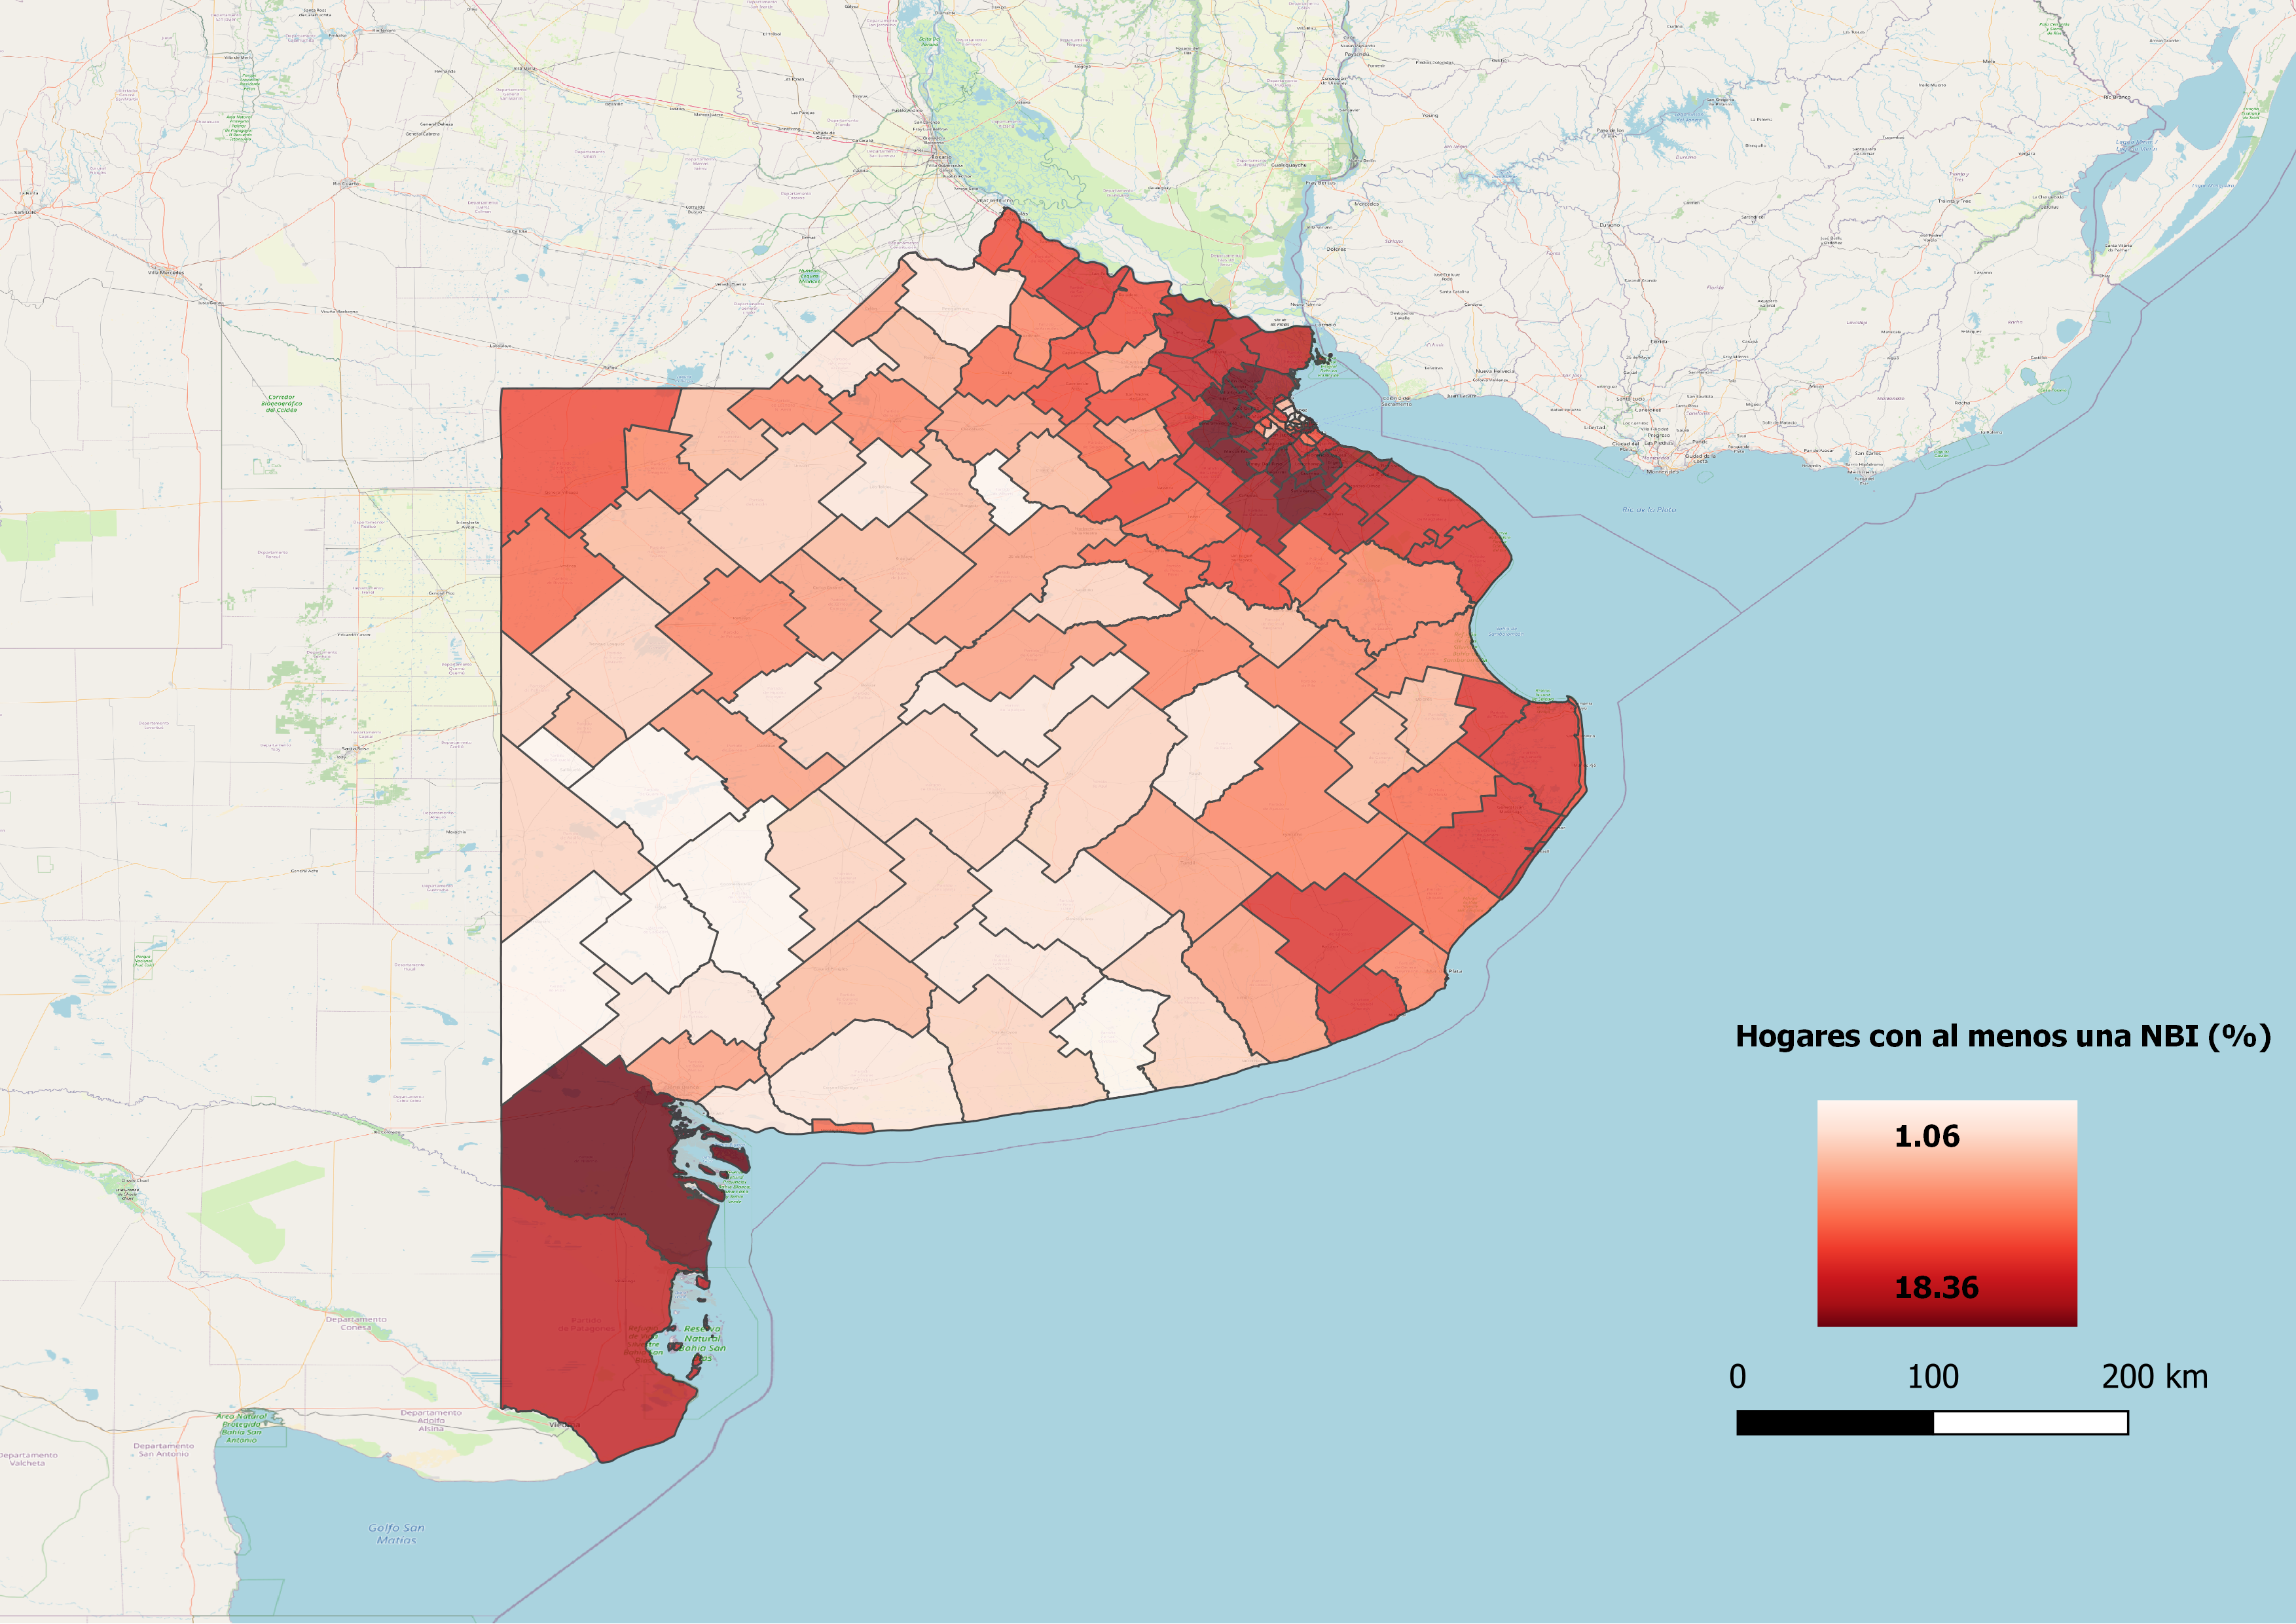
\includegraphics[scale=0.45]{imgs/NBI.png}
    \label{fig2}
\caption{Mapa de porcentaje de hogares con al menos una necesidad básica insatisfecha según departamento de la provincia de Buenos Aires}
\end{figure}
\end{document}
